\documentclass[12pt]{article}
\usepackage[russian]{babel}
\usepackage{geometry}

\usepackage{graphicx} % вставка изображений
\usepackage{caption} % описание изображений

%различные цветовые модели
\usepackage[usenames]{color}
\usepackage[dvipsnames,table]{xcolor}
\usepackage{colortbl}

\usepackage{tikz}
\usetikzlibrary{shapes, arrows}
\usepackage{varwidth}
\usepackage{ifthen}

\usepackage{multicol} % вставка изображений в две колонки
\usepackage{makecell} % вставка изображений в две колонки


%циклы foreach в tikz и создание переменных внутри этого окружения
\usepackage{pgffor}
\usepackage{pgfmath}

\usepackage{xifthen}

\usepackage{afterpage}

\usepackage{amssymb}
\usepackage{amsmath}

\usepackage{hyperref}

\usepackage[utf8]{inputenc}

\tikzstyle{connector} = [draw, -latex']
\tikzstyle{line} = [draw, -]
\tikzstyle{dashed} = [draw, -, dash pattern=on 5pt off 5pt]


\usepackage{listings}
\usepackage{listingsutf8}
\usepackage[T2A]{fontenc}
\newcommand{\listingsttfamily}{\usefont{T2A}{PTMono-TLF}{m}{n}}

\lstset{
	language=C,                % choose the language of the code
	numbers=left,                   % where to put the line-numbers
	stepnumber=1,                   % the step between two line-numbers.        
	numbersep=5pt,                  % how far the line-numbers are from the code
	backgroundcolor=\color{black},  % choose the background color. You must add \usepackage{color}
	commentstyle=\color{Gray},
	basicstyle=\listingsttfamily\color{Gray},
	keywordstyle=\color{BurntOrange},
	stringstyle=\color{YellowGreen},
	showspaces=false,               % show spaces adding particular underscores
	showstringspaces=false,         % underline spaces within strings
	showtabs=false,                 % show tabs within strings adding particular underscores
	tabsize=4,                      % sets default tabsize to 2 spaces
	captionpos=b,                   % sets the caption-position to bottom
	breaklines=true,                % sets automatic line breaking
	breakatwhitespace=true,         % sets if automatic breaks should only happen at whitespace
	title=\lstname, 
	inputencoding=utf8,                % show the filename of files included with \lstinputlisting;
	extendedchars=\true,
	keepspaces=true
}

\geometry{top=2cm, bottom=2cm, left=3cm, right=1.5cm}
\textheight=24cm
\textwidth=18cm
\flushbottom 

\oddsidemargin=0pt 
\topmargin=-1.5cm 
\parskip=0.25cm
\parindent=24pt 

\tolerance=2000 

\setcounter{secnumdepth}{0}

\begin{document}
	\begin{center}
		{\parskip=1cm
			МИНИСТЕРСТВО НАУКИ И ВЫСШЕГО ОБРАЗОВАНИЯ РОССИЙСКОЙ ФЕДЕРАЦИИ
			
			ФЕДЕРАЛЬНОЕ ГОСУДАРСТВЕННОЕ БЮДЖЕТНОЕ ОБРАЗОВАТЕЛЬНОЕ УЧРЕЖДЕНИЕ ВЫСШЕГО ОБРАЗОВАНИЯ
			
			{\bf«БЕЛГОРОДСКИЙ ГОСУДАРСТВЕННЫЙ ТЕХНОЛОГИЧЕСКИЙ УНИВЕРСИТЕТ им. В. Г. Шухова»\\(БГТУ им. В. Г. Шухова)}
			
			\begin{figure}[bh]
				\noindent\centering{
					
\includegraphics[width=100mm]{images/start_logo.png}
					\captionsetup{labelformat=empty}
				}
			\end{figure}
			Кафедра программного обеспечения вычислительной техники и автоматизированных систем
		}
		
		{\Large 
			\vspace{1cm}
			{\parskip=0.25cm 
				{\bf Лабораторная работа №3.4}
				
				по дисциплине: «Дискретная математика»
				
				по теме: {\bf Упорядоченные множества }
			}
		}
	\end{center}	
	\begin{flushleft}
		{\leftskip=10cm
			{\vspace{3cm} Выполнил/a: ст. группы ПВ-231}
			
			Чупахина София Александровна
			
			Проверил: Рязанов Юрий Дмитриевич
			
		}
	\end{flushleft}
	\begin{center}
		{\parskip=3cm Белгород, 2024}
	\end{center}
	\newpage

	{\Large \bf Вариант 6}
	 
	$A=\{(a, b) \Big| a_x - b_x < a_y - b_y\} $
	
	\tableofcontents
	\newpage
	
	\section{Задание 1}
	\label{task1}
	{\bf Текст задания:} Написать программы, формирующие матрицы отношений в соответствии с вариантом задания (табл. 3), на множествах $М1$ и $М2$. Определить свойства отношения. Если отношение не обладает свойством порядка, то выполнить следующий вариант заданий.
	
	Библиотека, разработанная ранее для работы с отношениями, предполагала, что отношения будут строиться на отрезке множества натуральных чисел, то есть на множестве $M$ с элементами --- числами от 1 до $|M|$. В нашем же случае отношения будут строиться на множествах точек. Вместо того, чтобы переписывать библиотеку дл работы с произвольным типом, в том числе для структуры <<точка>>, присвоим каждой точке из исходных множеств порядковый номер, и создадим отношения уже на множестве порядковых номеров точек.
	
	\begin{tikzpicture}{line width=3pt}
		\draw[step=1.5] (-3,-3) grid (3, 3);
		\draw[connector] (0, -3.5) -- (0, 3.5);
		\draw[connector] (-3.5, 0) -- (3.5, 0);
		
		\foreach \x in {-1, 0, 1} {
			\foreach \y in {-1, 0, 1} {
				\draw[black, line width=2pt] (1.5*\x, 1.5*\y) circle (4pt);
				\pgfmathsetmacro\val{int((\y+1)*3+\x + 2)} 
				\draw[red] (1.5*\x, -1.5*\y+0.5) node[fill=White]{\val};
			}
		};
		
		\draw[step=1.5] (5.75, -3) grid (12, 3);
		\draw[connector] (9, -3.5) -- (9, 3.5);
		\draw[connector] (5.5, 0) -- (12.5, 0);
		
	
		\foreach \x in {-1, 0, 1} {
			\foreach \y in {-1, 0, 1} {
				\draw[black, line width=2pt] (1.5*\x + 9, 1.5*\y) circle (4pt);
				\pgfmathsetmacro\val{int((\y+1)*3+\x + 2 + 1*(\y+2))} 
				\draw[red] (1.5*\x + 9, -1.5*\y+0.5) node[fill=White]{\val};
			}
		};
		
		\draw[black, line width=2pt] (6, 0) circle (4pt);
		\draw[black, line width=2pt] (12, 0) circle (4pt);
		\draw[black, line width=2pt] (9, 3) circle (4pt);
		\draw[black, line width=2pt] (9, -3) circle (4pt);
		\draw[red] (6, 0+0.5) node[fill=White]{5};
		\draw[red] (12, 0+0.5) node[fill=White]{9};
		\draw[red] (9, 3+0.5) node[fill=White]{1};
		\draw[red] (9, -3+0.5) node[fill=White]{13};
	\end{tikzpicture}
	
	Затем в файле C зададим структуру <<точка>>, имеющую два поля с целыми значениями: координаты x и y. Объявив как константы мощности множеств $M_1$ и $M_2$ (9 и 13 соответственно), создадим одноименные массивы, хранящие точки в том же порядке, в котором мы пронумеровали их на рисунке выше. Далее функция createForVariant6, принимающая как аргументы указатель на начало такого массива точек и его длину, перебирает все возможные пары точек в этом массиве, и если их координаты отвечают условию, заданному для варианта 6, то в отношение добавляется пара из порядковых номеров этих точек. Результирующее отношение и возвращается функцией. В теле функции main() остается только сохранить результат выполнения функции для массивов M1 и M2 (и их длин) и вывести матрицы полученных отношений на экран.
	
	\lstinputlisting[linerange={1-40, 130-143, 158}]{ordered_sets/ordered_sets_main.c} 
	
	\parbox[с][80mm][t]{70mm}{
		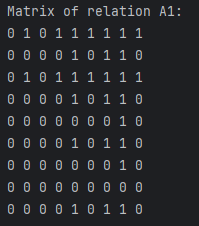
\includegraphics[width=65mm]{images/matrix1.png}
	}
	\hspace{2cm}
	\parbox[с][80mm][c]{60mm}{
		\begin{tabular} {c c c c c c c c c}
			0 & 1 & 0 & 1 & 1 & 1 & 1 & 1 & 1 \\
			0 & 0 & 0 & 0 & 1 & 0 & 1 & 1 & 0 \\
			0 & 1 & 0 & 1 & 1 & 1 & 1 & 1 & 1 \\
			0 & 0 & 0 & 0 & 1 & 0 & 1 & 1 & 0 \\
			0 & 0 & 0 & 0 & 0 & 0 & 0 & 1 & 0 \\
			0 & 0 & 0 & 0 & 1 & 0 & 1 & 1 & 0 \\
			0 & 0 & 0 & 0 & 0 & 0 & 0 & 1 & 0 \\
			0 & 0 & 0 & 0 & 0 & 0 & 0 & 0 & 0 \\
			0 & 0 & 0 & 0 & 1 & 0 & 1 & 1 & 0 \\
		\end{tabular}
	}
	
	\parbox[с][90mm][t]{70mm}{
		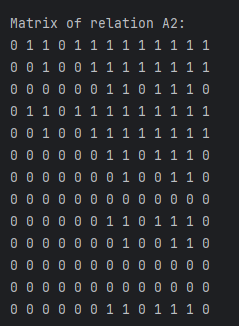
\includegraphics[width=65mm]{images/matrix2.png}
	}
	\hspace{2cm}
	\parbox[с][90mm][c]{60mm}{
		\begin{tabular} {c c c c c c c c c c c c c }
			0 & 1 & 1 & 0 & 1 & 1 & 1 & 1 & 1 & 1 & 1 & 1 & 1 \\
			0 & 0 & 1 & 0 & 0 & 1 & 1 & 1 & 1 & 1 & 1 & 1 & 1 \\
			0 & 0 & 0 & 0 & 0 & 0 & 1 & 1 & 0 & 1 & 1 & 1 & 0 \\
			0 & 1 & 1 & 0 & 1 & 1 & 1 & 1 & 1 & 1 & 1 & 1 & 1 \\
			0 & 0 & 1 & 0 & 0 & 1 & 1 & 1 & 1 & 1 & 1 & 1 & 1 \\
			0 & 0 & 0 & 0 & 0 & 0 & 1 & 1 & 0 & 1 & 1 & 1 & 0 \\
			0 & 0 & 0 & 0 & 0 & 0 & 0 & 1 & 0 & 0 & 1 & 1 & 0 \\
			0 & 0 & 0 & 0 & 0 & 0 & 0 & 0 & 0 & 0 & 0 & 0 & 0 \\
			0 & 0 & 0 & 0 & 0 & 0 & 1 & 1 & 0 & 1 & 1 & 1 & 0 \\
			0 & 0 & 0 & 0 & 0 & 0 & 0 & 1 & 0 & 0 & 1 & 1 & 0 \\
			0 & 0 & 0 & 0 & 0 & 0 & 0 & 0 & 0 & 0 & 0 & 0 & 0 \\
			0 & 0 & 0 & 0 & 0 & 0 & 0 & 0 & 0 & 0 & 0 & 0 & 0 \\
			0 & 0 & 0 & 0 & 0 & 0 & 1 & 1 & 0 & 1 & 1 & 1 & 0 \\
			\end{tabular}
	}
	
	Нетрудно заметить, что также для каждого из отношений вызывается функция, выводящая на экран основные и производные свойства этих отношений. В этот раз мы работаем только с матрицами отношений, в то время как доказательство наличия у отношения таких ключевых для данной работы свойств, как транзитивность и антитранзитивность, лишь по матрицам весьма затруднительно. Поэтому прибегнем к помощи ранее написанной функции.
	
	\newpage
	
	\begin{figure}[bh]
		\noindent\centering{
			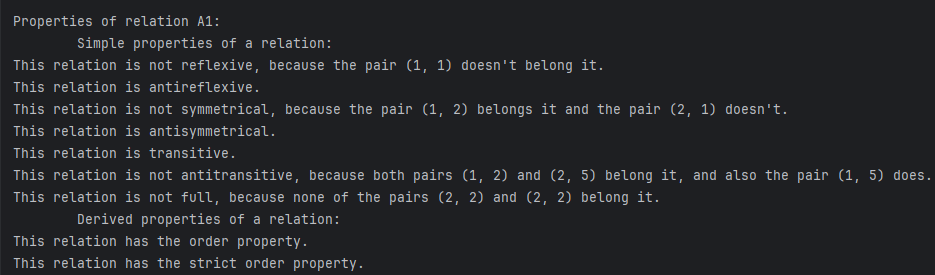
\includegraphics[width=180mm]{images/properties1.png}
			\captionsetup{labelformat=empty}
		}
	\end{figure}
	
	\begin{figure}[bh]
		\noindent\centering{
			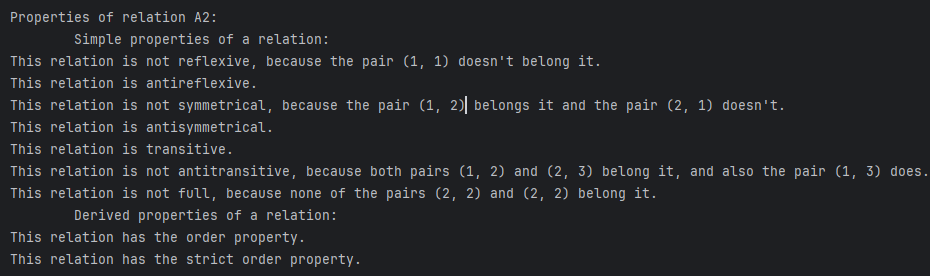
\includegraphics[width=180mm]{images/properties2.png}
			\captionsetup{labelformat=empty}
		}
	\end{figure}
	
	Оба полученных отношения не рефлексивны, но антирефлексивны, не симметричны, но антисимметричны, транзитивны, но не антитразитивны, не полны. Вследствие своей антисимметричности и транзитивности они обладают свойством порядка, а вследствие своей антирефлексивности также свойством строгого порядка.
	
	Поскольку оба отношения обладают свойством порядка, это позволяет нам перейти к следующему заданию.
	
	\section{Задание 2}
	\label{task2}
	
	{\bf Текст задания:} Написать программы, формирующие матрицы отношения доминирования по матрицам отношения порядка. 
	
	Отношение доминирования может быть получено над любым отношением порядка $\le$. В нем, помимо стандартных свойств отношения порядка, соблюдается условие, что для любых $x$ и $y$, если $x \le y$, не существует такого $z$, что $x \le z \le y$, что позволяет впоследствии выстроить между элементами некую иерархию (это отражено в названии).
	
	Также над любым отношением порядка можно получить отношение строгого порядка. Если отношение порядка по определению обладает свойствами антисимметричности и транзитивности, то отношение строгого порядка $<$ обладает также и свойством антирефлексивности. Значит, его можно получить из отношения порядка, вычтя из него главную диагональ: $< =  \le - I$ (как мы помним, как $I$ обозначается тождественное отношение, $I = \{(x, x) \Big| x \in A\}$).
	
	Отношение доминирования же находится как разность самого отношения строгого порядка и его квадрата: $\triangleleft = < - <^2$
	
	В нашем случае оба полученных отношения уже являются отношениями строгого порядка, но чтобы сделать наш код более универсальным и применимым для других отношений в дальнейшем (если это будет необходимо), позаботимся о том, чтобы функция преобразования отношения порядка в отношение строгого порядка также присутствовала.
	
	\lstinputlisting[linerange={41-51, 130-134, 144-150, 158}]{ordered_sets/ordered_sets_main.c} 
	
	\newpage

	Матрицы полученных отношений доминирования будут иметь следующий вид:
	
	\parbox[с][70mm][t]{70mm}{
		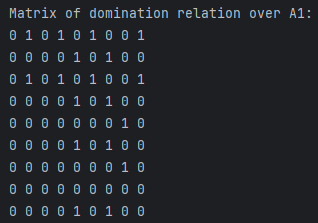
\includegraphics[width=85mm]{images/dom1.png}
	}
	\hspace{2cm}
	\parbox[с][70mm][c]{60mm}{
		\begin{tabular} {c c c c c c c c c}
			0 & 1 & 0 & 1 & 0 & 1 & 0 & 0 & 1 \\
			0 & 0 & 0 & 0 & 1 & 0 & 1 & 0 & 0 \\
			0 & 1 & 0 & 1 & 0 & 1 & 0 & 0 & 1 \\
			0 & 0 & 0 & 0 & 1 & 0 & 1 & 0 & 0 \\
			0 & 0 & 0 & 0 & 0 & 0 & 0 & 1 & 0 \\
			0 & 0 & 0 & 0 & 1 & 0 & 1 & 0 & 0 \\
			0 & 0 & 0 & 0 & 0 & 0 & 0 & 1 & 0 \\
			0 & 0 & 0 & 0 & 0 & 0 & 0 & 0 & 0 \\
			0 & 0 & 0 & 0 & 1 & 0 & 1 & 0 & 0 \\
		\end{tabular}
	}
	
	\parbox[с][90mm][t]{70mm}{
		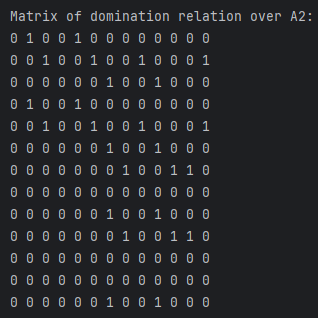
\includegraphics[width=85mm]{images/dom2.png}
	}
	\hspace{2cm}
	\parbox[с][90mm][c]{60mm}{
		\begin{tabular} {c c c c c c c c c c c c c }
			0 & 1 & 0 & 0 & 1 & 0 & 0 & 0 & 0 & 0 & 0 & 0 & 0 \\
			0 & 0 & 1 & 0 & 0 & 1 & 0 & 0 & 1 & 0 & 0 & 0 & 1 \\
			0 & 0 & 0 & 0 & 0 & 0 & 1 & 0 & 0 & 1 & 0 & 0 & 0 \\
			0 & 1 & 0 & 0 & 1 & 0 & 0 & 0 & 0 & 0 & 0 & 0 & 0 \\
			0 & 0 & 1 & 0 & 0 & 1 & 0 & 0 & 1 & 0 & 0 & 0 & 1 \\
			0 & 0 & 0 & 0 & 0 & 0 & 1 & 0 & 0 & 1 & 0 & 0 & 0 \\
			0 & 0 & 0 & 0 & 0 & 0 & 0 & 1 & 0 & 0 & 1 & 1 & 0 \\
			0 & 0 & 0 & 0 & 0 & 0 & 0 & 0 & 0 & 0 & 0 & 0 & 0 \\
			0 & 0 & 0 & 0 & 0 & 0 & 1 & 0 & 0 & 1 & 0 & 0 & 0 \\
			0 & 0 & 0 & 0 & 0 & 0 & 0 & 1 & 0 & 0 & 1 & 1 & 0 \\
			0 & 0 & 0 & 0 & 0 & 0 & 0 & 0 & 0 & 0 & 0 & 0 & 0 \\
			0 & 0 & 0 & 0 & 0 & 0 & 0 & 0 & 0 & 0 & 0 & 0 & 0 \\
			0 & 0 & 0 & 0 & 0 & 0 & 1 & 0 & 0 & 1 & 0 & 0 & 0 \\
		\end{tabular}
	}
	
	\section{Задание 3}
	\label{task3}

	{\bf Текст задания:} Написать программу, реализующую алгоритм топологической сортировки по матрице отношения доминирования.
	
	Принимаясь за реализацию этого алгоритма в программном виде, стоит задуматься: будет ли храниться где-то полученный результат --- сортировка элементов множества по уровням? Конечно, можно ограничиться обычным выводом, без сохранения результата. Однако подумав чуть дольше, мы можем провести аналогию между этой задачей и задачей хранения классов эквивалентности в прошлой лабораторной работе. Нам также необходимо разбить множество на непересекающиеся подмножества, при этом такие, что их объединение дает исходное множество. Ведь очевидно, что каждый элемент принадлежит хотя бы какому-то уровню и при этом не может принадлежать двум уровням сразу.
	
	Таким образом, мы можем скопировать в программу структуру splitting и функции инициализации и вывода для нее без значительных изменений и переименований (разбиение множества на уровни, а не на классы эквивалентности, все еще остается разбиением). При создании структуры требуется параметр max\_value, мощность множества, разбиение которого будет храниться. Выделяется память для хранения массива целых чисел длины max\_value, и все его элементы инициализируются нулями. В поле display будет храниться указатель на этот массив, а в поле max\_value --- одноименный входной параметр. При печати используется следующий алгоритм: сначала производится проход по массиву display, в ходе которого находится максимальный номер множества-элемента разбиения, max\_set. Затем в теле цикла for перебираются номера таких множеств от 1 до max\_set, и для каждого номера совершается проход по массиву display. Если на некоторой его позиции хранится текущий номер, значит, соответствующий элемент исходного множества входит в множество-элемент разбиения. Этот элемент выводится на экран. До прохода по массиву выводится открывающая скобка <<\{>>, после прохода по массиву --- закрывающая <<\}>>, для обособления отдельных множеств-элементов разбиения. Перед основной частью алгоритма и после нее будут выводиться квадратные скобки; квадратные --- потому что в нашем случае некорректно называть результат множеством. Порядок множество внутри разбиения имеет значение: в каждой последовательности элементы первого множества относятся к самому низкому, первому уровню, элементы последнего множества --- к самому высокому уровню.
	
	Алгоритм же сортировки мы реализуем в функции getLevelsSet, которая и возвращает структуру типа splitting. Вначале создается разбиение l для хранения уровней, массив w\_array для хранения суммы столбцов матрицы отношения, задается начальное количество уровней, равное 1, и стартовое значение i = -1. С помощью двух вложенных циклов для каждого столбца матрицы считается сумма элементов и сохраняется на соответствующей позиции массива w\_array. Затем инициализируется переменная flag, и ее значение определяется в цикле, после прохода по массиву в котором становится понятно, есть ли в нем хотя бы один неотрицательный элемент. Если есть, запускается основная часть алгоритма: поиск в массиве w\_array нулей и замена их на i; поиск i в массиве w\_array и вычитание из него строк матрицы с номерами, соответствующими индексам элементов i в массиве; уменьшение i на 1, увеличение количества уровней на 1, изменение значения flag (выполнение алгоритма продолжается, пока flag истинна и в массиве w\_array есть хотя бы один неотрицательный элемент).
	
	\lstinputlisting[linerange={53-133, 144-158}]{ordered_sets/ordered_sets_main.c} 
	
	\newpage
	
	На экран будут выведены следующие последовательности множеств.
	
	\begin{figure}[bh]
		\noindent\centering{
			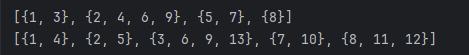
\includegraphics[width=150mm]{images/levels.png}
			\captionsetup{labelformat=empty}
		}
	\end{figure}
	
	\section{Задание 4}
	\label{task4}

	{\bf Текст задания:} Изобразить диаграмму Хассе отношения доминирования на множествах $M_1$ и $M_2$. 
	
	Опираясь на полученные топологические сортировки, мы можем разбить элементы по уровням, а сверяясь с матрицами соответствующих отношений доминирования, провести дуги от элементов нижних уровней к элементам верхних.
	
	Диаграмма Хассе на отношении доминирования над множеством $M_1$ будет выглядеть следующим образом:
	
	
	\begin{tikzpicture}{line width=3pt}
		\node[circle, draw=black, minimum height=1.75cm] at (-4.5, -5) (knot1) {\makecell[c]{1 \\ (-1, 1)}};
		\node[circle, draw=black, minimum height=1.75cm] at (4.5, -5) (knot3) {\makecell[c]{3 \\ (1, 1)}};
		
		\node[circle, draw=black, minimum height=1.75cm] at (-4.5, -1) (knot2) {\makecell[c]{2 \\ (0, 1)}};
		\node[circle, draw=black, minimum height=1.75cm] at (-1.5, -1) (knot4) {\makecell[c]{4 \\ (-1, 0)}};
		\node[circle, draw=black, minimum height=1.75cm] at (1.5, -1) (knot6) {\makecell[c]{6 \\ (1, 0)}};
		\node[circle, draw=black, minimum height=1.75cm] at (4.5, -1) (knot9) {\makecell[c]{9 \\ (1, -1)}};
		
		\node[circle, draw=black, minimum height=1.75cm] at (-4.5, 3) (knot5) {\makecell[c]{5 \\ (0, 0)}};
		\node[circle, draw=black, minimum height=1.75cm] at (4.5, 3) (knot7) {\makecell[c]{7 \\ (-1, -1)}};
		
		\node[circle, draw=black, minimum height=1.75cm] at (0, 6) (knot8) {\makecell[c]{8 \\ (0, -1)}};
		
		\foreach \x in {1, 3} {
			\foreach \y in {2, 4, 6, 9} {
				\path[connector, line width = 1.25pt] (knot\x) -- (knot\y);							
			}
		}
		
		\foreach \x in {2, 4, 6, 9} {
			\foreach \y in {5, 7} {
				\path[connector, line width = 1.25pt] (knot\x) -- (knot\y);							
			}
		}
		
		\foreach \x in {5, 7} {
				\path[connector, line width = 1.25pt] (knot\x) -- (knot8);							
		}
	\end{tikzpicture}
	
	\newpage
	
	А диаграмма Хассе на отношении доминирования над множеством $M_2$ --- следующим образом:
	
	\begin{tikzpicture}{line width=3pt}
		\node[circle, draw=black, minimum height=1.75cm] at (-4.5, -5) (knot1) {\makecell[c]{1 \\ (0, 2)}};
		\node[circle, draw=black, minimum height=1.75cm] at (4.5, -5) (knot4) {\makecell[c]{4 \\ (1, 1)}};
		
		
		\node[circle, draw=black, minimum height=1.75cm] at (-4.5, -2) (knot2) {\makecell[c]{2 \\ (-1, 1)}};
		\node[circle, draw=black, minimum height=1.75cm] at (4.5, -2) (knot5) {\makecell[c]{5 \\ (-2, 0)}};
		
		\node[circle, draw=black, minimum height=1.75cm] at (-4.5, 2) (knot3) {\makecell[c]{3 \\ (0, 1)}};
		\node[circle, draw=black, minimum height=1.75cm] at (-1.5, 2) (knot6) {\makecell[c]{6 \\ (-1, 0)}};
		\node[circle, draw=black, minimum height=1.75cm] at (1.5, 2) (knot9) {\makecell[c]{9 \\ (2, 0)}};
		\node[circle, draw=black, minimum height=1.75cm] at (4.5, 2) (knot13) {\makecell[c]{13 \\ (0, -2)}};
		
		\node[circle, draw=black, minimum height=1.75cm] at (-4.5, 6) (knot7) {\makecell[c]{7 \\ (0, 0)}};
		\node[circle, draw=black, minimum height=1.75cm] at (4.5, 6) (knot10) {\makecell[c]{10 \\ (-1, -1)}};
		
		\node[circle, draw=black, minimum height=1.75cm] at (-4.5, 10) (knot8) {\makecell[c]{8 \\ (1, 0)}};
		\node[circle, draw=black, minimum height=1.75cm] at (0, 10) (knot11) {\makecell[c]{11 \\ (0, -1)}};
		\node[circle, draw=black, minimum height=1.75cm] at (4.5, 10) (knot12) {\makecell[c]{12 \\ (1, -1)}};
		
		\foreach \x in {1, 4} {
			\foreach \y in {2, 5} {
				\path[connector, line width = 1.25pt] (knot\x) -- (knot\y);							
			}
		}
		
		\foreach \x in {2, 5} {
			\foreach \y in {3, 6, 9, 13} {
				\path[connector, line width = 1.25pt] (knot\x) -- (knot\y);							
			}
		}
		
		\foreach \x in {3, 6, 9, 13} {
			\foreach \y in {7, 10} {
				\path[connector, line width = 1.25pt] (knot\x) -- (knot\y);	
			}						
		}
		
		\foreach \x in {7, 10} {
			\foreach \y in {8, 11, 12} {
				\path[connector, line width = 1.25pt] (knot\x) -- (knot\y);	
			}						
		}
	\end{tikzpicture}
	
	\section{Задание 5}
	\label{task5}
	
	{\bf Текст задания:} Найти минимальные и максимальные элементы множеств $M_1$ и $M_2$. 
	
	Минимальными элементами в каждом отношении порядка будут те элементы, которые принадлежат наиболее низкому уровню в соответствующем отношении доминирования; максимальными --- все те, которые принадлежат наиболее высокому уровню.
	
	Проанализировав диаграмму отношения доминирования на множестве $M_1$, составленную в задании 4, мы можем увидеть, что	для него минимальными элементами будут элементы 1 и 3, соответствующие точкам $(-1, 1)$ и $(1, 1)$. Максимальный же элемент будет только один --- 8, соответствующий точке $(0, -1)$. Это можно проверить, проанализировав соответствующие {\it столбцы} матрицы исходного отношения для минимальных элементов и {\it строки} для максимальных. Анализируя {\it столбец} элемента $x$, мы анализируем все пары вида $(a, x)$. Если столбец содержит хотя бы одну единицу (кроме как в строке, соответствующей этому же элементу, если само по себе отношение не обладает свойством строгого порядка), это значит, что для элемента $x$ существует элемент $a$, меньший его. Если же столбец не содержит единиц, значит, любой другой элемент больше $x$ либо не сравним с ним. И наоборот, анализируя {\it строку} элемента $x$, мы анализируем все пары вида $(x, a)$. Если столбец содержит хотя бы одну единицу, это значит, что для элемента $x$ существует элемент $a$, больший его; иначе остальные элементы либо меньше $x$, либо не сравнимы с ним. Эти свойства соответствуют условиям, которым должны обладать минимальные и максимальные элементы. И если мы просмотрим строки максимальных элементов и столбцы минимальных, мы увидим, что единиц они и впрямь не содержат. Значит, они были выбраны верно.
	
	Перейдя к отношению на множестве $M_2$, мы можем сказать, что минимальными элементами для него будут элементы 1 и 4, соответствующие точкам $(0, 2)$ и $(1, 1)$. Максимальных же элементов будет три --- 8, 11 и 12, соответствующие точкам $(1, 0)$, $(0, -1)$ и $(1, -1)$. Точно так же {\it столбцы} минимальных элементов и {\it строки} максимальных в исходной матрице содержат только нули. 
		
	\section{Задание 6}
	\label{task6}
		
	{\bf Текст задания:} Найти, если существуют, наименьший и наибольший элементы множеств $M_1$ и $M_2$.
	
	Если некоторое отношение доминирования имеет на своем наиболее низком уровне только один элемент, то он и будет наименьшим в соответствующем отношении порядка. И наоборот, если на наиболее высоком уровне отношения доминирования находится только один элемент, то он и будет наибольшим в соответствующем отношении порядка.
	
	Согласно наблюдениям в задании 5, на нижнем уровне диаграммы отношения на множестве $M_1$ находятся два элемента. Все они являются минимальными, но ни один из них нельзя назвать наименьшим, потому что между собой они несравнимы. Это заключение можно подтвердить тем похожим, но все-таки отличающимся анализом матрицы исходного отношения. В {\it строках} матрицы, соответствующих этим элементам, содержится больше одного нуля --- то есть существуют элементы, с которыми они несравнимы, кроме самих себя (это не могут быть элементы, которые меньше данных, потому что в задании 5 мы выяснили: элементы первого уровня минимальны). На верхнем же уровне диаграммы находится только один элемент, 8 (точка $(0, -1)$), и его можно назвать наибольшим. Это подтверждается, если мы проанализируем {\it столбец} матрицы, соответствующий этому элементу: он содержит только 1 ноль, знак того, что элемент не сравним сам с собой.
	
	Произведем аналогичные рассуждения для отношения на множестве $M_2$. На нижнем уровне диаграммы отношения доминирования находятся два элемента. Они также являются лишь минимальными, но не наименьшими, и в соответствующих {\it строках} матрицы исходного отношения больше одного нуля, что показывает, что существуют элементы, с которыми они не сравнимы. На верхнем же уровне диаграммы находятся три элемента, максимальных, но не наибольших. Это подтверждается анализом {\it столбцов} матрицы, соответствующих этим элементам: они содержат больше одного нуля, что значит, что существуют элементы, с которыми они несравнимы.
	
	Подведем итоги: в отношении на множестве $M_1$ нет наименьшего элемента, но есть наибольший элемент: 8 точка $(0, -1)$ с порядковым номером 8. В отношении на множестве $M_2$ не существует ни наименьшего, ни наибольшего элемента.
	
	\section{Вывод}
	\label{final}
	
	Если некоторое отношение обладает свойством порядка или зависящими от него свойствами строго или нестрого, линейного строгого или нестрогого порядка, то между его элементами возникают более глубокие логические связи и свойства. Среди элементов исходного множества для такого отношения всегда существуют максимальные и минимальные. Необязательно, но возможно существование наибольшего и наименьшего элемента, причем наибольший и наименьший элемент в множестве может быть только один. Также над исходным отношением порядка всегда можно построить отношение строгого порядка, а следом --- и отношение доминирования. Для отношения доминирования, в свою очередь, элементы можно разбить на уровни --- такое разбиение называется топологической сортировкой; ее получение помогает в дальнейшем быстро находит минимальные и максимальные, наибольший и наименьший (при их наличии) элементы для исходного отношения порядка. В ходе лабораторной работы научились создавать для отношения порядка отношение доминирования, запрограммировали алгоритм получения топологической сортировки по отношению доминирования, научились строить диаграммы Хассе для отношений доминирования и искать максимальные и минимальные, наибольший и наименьший элементы.

\end{document}